\documentclass{article}%
\usepackage[T1]{fontenc}%
\usepackage[utf8]{inputenc}%
\usepackage{lmodern}%
\usepackage{textcomp}%
\usepackage{lastpage}%
\usepackage[head=40pt,margin=0.5in,bottom=0.6in]{geometry}%
\usepackage{graphicx}%
%
\title{\textbf{Contaminación en el hospital precipitó muerte de dos niñas}}%
\author{Oriana Camacho Bastos | obastos@el{-}nacional.com}%
\date{23/11/2018}%
%
\begin{document}%
\normalsize%
\maketitle%
\textbf{URL: }%
http://www.el{-}nacional.com/noticias/sociedad/contaminacion{-}hospital{-}precipito{-}muerte{-}dos{-}ninas\_260778\newline%
%
\textbf{Periodico: }%
EN, %
ID: %
260778, %
Seccion: %
Sociedad\newline%
%
\textbf{Palabras Claves: }%
Salud, Caracas, Hospitales, Sociedad\newline%
%
\textbf{Derecho: }%
2.1%
, Otros Derechos: %
NO\_TIENE%
, Sub Derechos: %
2.1.1%
\newline%
%
\textbf{EP: }%
NO\newline%
\newline%
%
\textbf{\textit{El J. M. de los Ríos carece de medicinas e insumos, y la falta de mantenimiento de los tanques de agua afecta a los pacientes con enfermedades terminales}}%
\newline%
\newline%
%
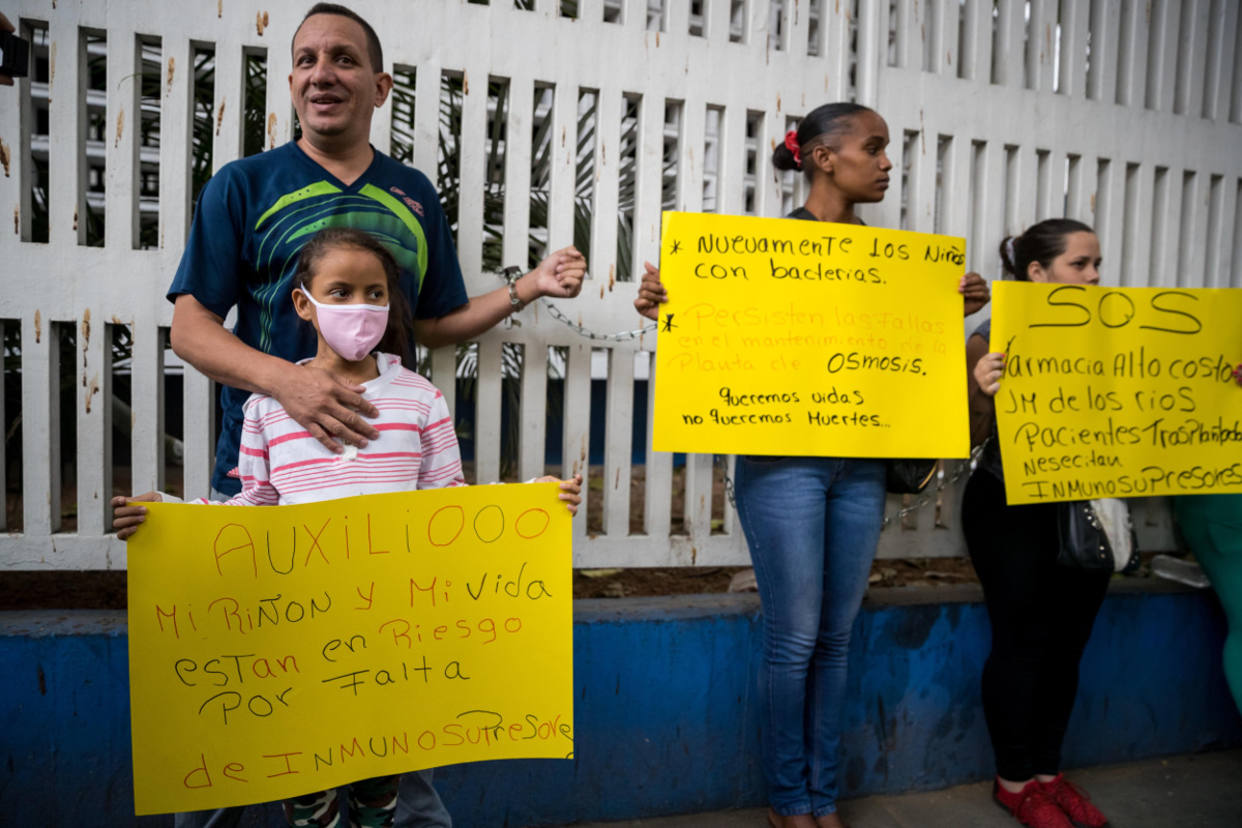
\includegraphics[width=300px]{133.jpg}%
\newline%
%
El Hospital J. M. de los Ríos está de luto desde el miércoles. En la mañana murió Frannly Herrera, una joven de 16 años de edad, que se encontraba hospitalizada en el área de Nefrología; y en horas de la tarde falleció Wilmely Mendoza, de 9 años de edad. Ambas se suman a los 18 menores que han perdido la vida en ese centro de salud infantil desde 2017. Katherine Martínez, presidente de Prepara Familia, aseguró que las niñas se encontraban en situación de emergencia, pero debido a que esa institución no recibe atención adecuada por parte del Estado, fueron víctimas de la contaminación y las carencias que allí se padecen.%
\newline%
%
“Se necesita la desinfección de los tanques de agua que surten al hospital y el mantenimiento de la planta de ósmosis que correspondía al mes de agosto, y aún no se ha realizado. A esto se agrega la falta de los antibióticos pues actualmente se suministran de manera irregular. Habíamos advertido que si no se realizaba un cambio en los tanques habría graves consecuencias para nuestros pequeños”, destacó.%
\newline%
%
También informó que el lunes falleció~Rolianmerys,~una niña de la Unidad de Hematología, con leucemia linfoblástica~aguda. “Esta pequeña no murió por lo delicado de su enfermedad, sino~producto del~tratamiento~que recibía el cual causó una infección bacteriana. Ellas estarían vivas si se hubiesen cumplido todos los protocolos que requiere el hospital”, dijo.%
\newline%
%
Aún se realizan averiguaciones sobre el deceso de las dos pequeñas de Nefrología, debido a que involucra las carencias de medicinas, suministros, contaminación e infecciones que sufre el centro de salud. Martínez manifestó que el Estado debe responder por estas muertes y todas la que han ocurrido en los últimos dos años. “Ellos son los únicos responsables de la vida y la salud de todos los niños del J. M. de los Ríos”.%
\newline%
%
El fallecimiento de las niñas ocurrió el miércoles 21, cuando se cumplieron 9 meses de la decisión de la Comisión Interamericana de Derechos Humanos,~que otorgó medidas de protección a los pacientes de Nefrología y ordenó al Estado a amparar la vida, integridad personal y salud de todos los pequeños que se encuentran hospitalizados en esa unidad, además de los de Oncología y Hematología. No obstante, este~sigue sin ejecutar la medida y sin responder a los problemas que agobian al centro asistencial infantil.%
\newline%
%
CIFRAS%
\newline%
%
9 Meses han transcurrido desde que la CIDH dictó medidas de protección a los pequeños pacientes porque el Estado no responde a la emergencia que atraviesa el hospital%
\newline%
%
\end{document}